\documentclass[12pt]{report}

%-----------------------------------------------------------------
% LaTeX template for a Bachelor Capstone Project Report of the COLLEGE OF Mechatronics, Ha Noi University of Science and Technology

% Prepared and Designed By: Van Dinh Nguyen. 
% Date published: August 25, 2023
% For any comments: dinh.nv2@vinuni.edu.vn

\usepackage{subfigure}
\usepackage[utf8]{vietnam}
\usepackage[left=3.5cm, right=2.5cm, top=2cm, bottom=2cm]{geometry}
\usepackage{fancybox,graphicx}
\usepackage{mathrsfs} 
\usepackage{array} % Sử dụng gói array để điều chỉnh định dạng cột trong bảng
\usepackage{booktabs} % Sử dụng gói booktabs để sử dụng các lệnh \toprule, \midrule và \bottomrule
% \usepackage{fontspec}
\usepackage{tikz} %Vẽ sơ đồ khối
\renewcommand{\baselinestretch}{1.5}
% \setmainfont{Times New Roman}
\usepackage{titlesec}

\titleformat{\chapter}[display]
{\normalfont\huge\bfseries}{\chaptertitlename\ \thechapter}{20pt}{\Huge}

\titlespacing*{\chapter}{0pt}{-10pt}{10pt} % Giảm khoảng cách trước và sau chương
\setlength{\headheight}{17.97171pt}

\usepackage{amsfonts}
\usepackage{longtable,array}
\usepackage{multirow}
\newlength\mylength
\newcolumntype{C}[1]{>{\centering\arraybackslash}p{#1}}
\usepackage[intlimits]{amsmath}
\usepackage{array}
\usepackage[unicode]{hyperref}
\usepackage{algorithm}
\usepackage{algorithmicx}
\makeatletter
\renewcommand{\ALG@name}{Thuật toán}
\makeatother
\usepackage{algpseudocode}
\usepackage{amsxtra,amssymb,latexsym,amscd,amsthm}
\usepackage{enumitem}
\usepackage{tikz}
\usetikzlibrary{shapes.geometric}
\usetikzlibrary{positioning,automata}
\usepackage{scrextend}
\usepackage{longfbox}

\usepackage{fancyhdr}
\pagestyle{fancy}
\lhead{}
\chead{}
% \lfoot{Kỹ thuật lập trình trong cơ điện tử}
\rfoot{ GVHD: Trương Công Tuấn}
\cfoot{\thepage}



\usepackage{xcolor}
\usepackage{listings}

\definecolor{mGreen}{rgb}{0,0.6,0}
\definecolor{mGray}{rgb}{0.5,0.5,0.5}
\definecolor{mPurple}{rgb}{0.58,0,0.82}
\definecolor{backgroundColour}{rgb}{0.95,0.95,0.92}

\lstdefinestyle{CStyle}{
	backgroundcolor=\color{backgroundColour},   
	commentstyle=\color{mGreen},
	keywordstyle=\color{magenta},
	numberstyle=\tiny\color{mGray},
	stringstyle=\color{mPurple},
	basicstyle=\footnotesize,
	breakatwhitespace=false,         
	breaklines=true,                 
	captionpos=b,                    
	keepspaces=true,                 
	numbers=left,                    
	numbersep=5pt,                  
	showspaces=false,                
	showstringspaces=false,
	showtabs=false,                  
	tabsize=2,
	language=C
}

\begin{document}

\thispagestyle{empty}
\thisfancypage{
	\setlength{\fboxsep}{0pt}
	\fbox}{}

\begin{center}
	
	{\fontsize{13pt}{1}\selectfont\textbf{TRƯỜNG ĐẠI HỌC BÁCH KHOA HÀ NỘI}}
	\\
	{\fontsize{13pt}{1}\selectfont\textbf{TRƯỜNG CƠ KHÍ}}
	\\		
	\textbf{--------------------  o0o  ---------------------}\\[1cm]
	
\includegraphics[scale=0.5]{image/BVP-logo bk-rgb.jpg} \\[1cm]
\textbf{{\LARGE VI XỬ LÝ}}\\[0.2cm]
\textbf{{\LARGE HỆ THỐNG ĐO SỬ DỤNG VI XỬ LÝ}}
\textbf{}\\[1cm]
\end{center}

\begin{flushleft}
\hspace{1.5 cm} \fontsize{14pt}{1}\textbf{ Giáo viên hướng dẫn:\hspace{0.4cm}{GVHD}}\\[0.5cm]
\hspace{1.5 cm} \textbf{ Sinh viên thực hiện:
\hspace{0.4cm}{  Nhóm 13:\\[0.2cm]}
\hspace{7.3 cm}{  Ngô Xuân Phong    - 20200461\\[0.2cm]}
\hspace{7.3 cm}{ Lê Công Minh      - 20205372\\[0.2cm]}
\hspace{7.3 cm}{ Trần Trung Thành  - 20205431\\[0.2cm]}
\hspace{7.3 cm}{ Vũ Minh Hoá       - 20205314\\}}

\end{flushleft}

% \vspace{}
\begin{center}
\textbf{{\normalsize Hà Nội - 7/2023}}\\
\end{center}

\tableofcontents

\newpage
\chapter*{Mở đầu}

Hệ thống phân loại sản phẩm bằng màu sắc đóng vai trò quan trọng trong quá trình tự động hóa và giám sát trong nhiều lĩnh vực công nghiệp và sản xuất. Bằng cách sử dụng cảm biến màu sắc và vi điều khiển Arduino, chúng ta có thể hiện thực một giải pháp thông minh để phân loại các sản phẩm dựa trên thông tin màu sắc của chúng.

Màu sắc là một thông tin quan trọng và dễ nhận diện trong hầu hết các loại sản phẩm. Hệ thống phân loại sản phẩm dựa trên màu sắc có thể được áp dụng trong ngành công nghiệp sản xuất, dệt may, đóng gói và nhiều ứng dụng khác. Việc sử dụng cảm biến màu sắc và Arduino cho phân loại sản phẩm giúp tăng cường hiệu suất, độ chính xác và giảm thiểu sự can thiệp của con người.

Trong bài báo cáo này, chúng ta sẽ trình bày về cấu trúc và hoạt động của hệ thống phân loại sản phẩm sử dụng cảm biến màu sắc và Arduino. Bài báo cáo bao gồm các thành phần chính của hệ thống, quy trình xử lý tín hiệu màu sắc, cách thức cài đặt và lập trình Arduino để điều khiển hệ thống, cùng với các thử nghiệm và kết quả đạt được.

Hi vọng rằng bài báo cáo này sẽ đem lại cái nhìn tổng quan về hệ thống phân loại sản phẩm sử dụng cảm biến màu sắc và Arduino, và hướng dẫn cụ thể cho việc triển khai một giải pháp phân loại sản phẩm thông minh và tiết kiệm thời gian trong các ứng dụng thực tế.


Chúng em xin cảm ơn thầy Trương Công Tuấn vì những giờ giảng dạy đầy nhiệt tình.  Nếu như trong báo cáo còn có những thiếu sót, kính mong thầy và các bạn nhiệt tình đóng góp ý kiến xây dựng để báo cáo ngày càng hoàn thiện hơn.
\chapter{TỔNG QUAN ĐỀ TÀI}

Trong thời đại công nghệ 4.0 đang phát triển mạnh mẽ, nhu cầu tự động hóa và tăng cường hiệu suất trong quá trình sản xuất và giám sát ngày càng trở nên quan trọng. Hệ thống phân loại sản phẩm dựa trên màu sắc là một ứng dụng tiêu biểu trong lĩnh vực tự động hóa và là một giải pháp hiệu quả để tối ưu hoá quy trình công nghiệp.

Đề tài này tập trung vào việc nghiên cứu và xây dựng hệ thống phân loại sản phẩm bằng màu sắc sử dụng cảm biến màu sắc và vi điều khiển Arduino. Cảm biến màu sắc được sử dụng để thu thập thông tin màu sắc của các sản phẩm trong quá trình sản xuất. Thông tin này sau đó sẽ được xử lý và phân loại bởi vi điều khiển Arduino.

Trong quá trình nghiên cứu và phát triển, chúng tôi sẽ tập trung vào các yếu tố quan trọng như độ chính xác, hiệu suất và tính ứng dụng của hệ thống. Các thuật toán xử lý tín hiệu màu sắc sẽ được tối ưu hóa để đảm bảo tính chính xác trong việc phân loại các sản phẩm với màu sắc khác nhau. Đồng thời, vi điều khiển Arduino sẽ được lập trình và điều chỉnh để thực hiện công việc phân loại một cách hiệu quả và nhanh chóng.

Hy vọng rằng kết quả của đề tài này sẽ đóng góp vào việc nâng cao năng suất và tối ưu hoá quy trình sản xuất trong nhiều lĩnh vực công nghiệp. Hệ thống phân loại sản phẩm bằng màu sắc sử dụng cảm biến màu sắc và Arduino hứa hẹn trở thành một công cụ hữu ích và tiết kiệm thời gian trong các ứng dụng thực tế.

\section{Giới hạn đề tài:}
Đề tài \textbf{Hệ thống phân loại sản phẩm bằng màu sắc sử dụng cảm biến màu sắc và Arduino} sẽ được giới hạn như sau:

\begin{enumerate}[itemsep=0pt, parsep=0pt]
    \item Tập trung vào phân loại màu sắc của các sản phẩm, không đi sâu vào các yếu tố khác như hình dạng hoặc kích thước 
    \item Nghiên cứu sử dụng cảm biến màu sắc để thu thập thông tin màu sắc của sản phẩm.
    \item Sử dụng vi điều khiển Arduino để xử lý thông tin màu sắc từ cảm biến và thực hiện quá trình phân loại sản phẩm.
    \item Nghiên cứu và triển khai các thuật toán xử lý tín hiệu màu sắc để phân loại sản phẩm dựa trên thông tin thu thập được.
    \item Thực hiện các thử nghiệm và đánh giá hiệu suất của hệ thống phân loại sản phẩm.
    \item Cải tiến và tối ưu hóa hệ thống để nâng cao hiệu suất và độ chính xác.
    \item Tạo ra môi trường thử nghiệm chính xác và đáng tin cậy để đánh giá và so sánh kết quả thực nghiệm.
    \item So sánh hệ thống phân loại sản phẩm dựa trên cảm biến màu sắc và Arduino với các phương pháp và giải pháp phân loại khác trong lĩnh vực tương tự.
\end{enumerate}
 
\section{Nhiệm vụ nghiên cứu:}
Trong đề tài \textbf{Hệ thống phân loại sản phẩm bằng màu sắc sử dụng cảm biến màu sắc và Arduino}, chúng ta sẽ thực hiện các nhiệm vụ nghiên cứu sau:

\begin{enumerate}[itemsep=0pt, parsep=0pt]
    \item Tìm hiểu và phân tích công nghệ cảm biến màu sắc.
    \item Nghiên cứu về vi điều khiển Arduino và khả năng xử lý dữ liệu màu sắc.
    \item Xác định yêu cầu hệ thống phân loại sản phẩm dựa trên thông tin màu sắc.
    \item Thiết kế mạch và giao tiếp cảm biến màu sắc với vi điều khiển Arduino.
    \item Lập trình vi điều khiển Arduino để thu thập thông tin màu sắc và phân loại sản phẩm.
    \item Cải tiến và tối ưu hóa hệ thống phân loại để nâng cao hiệu suất.
    \item Thiết lập môi trường thử nghiệm chính xác và đáng tin cậy.
    \item Viết báo cáo khoa học và thuyết trình kết quả nghiên cứu.
\end{enumerate}

\section{Ý nghĩa khoa học và thực tiễn}
\begin{enumerate}[itemsep=0pt, parsep=0pt]
    \item \textbf{Ứng dụng trong công nghiệp tự động hóa:} Đề tài đề xuất một giải pháp phân loại sản phẩm thông minh dựa trên thông tin màu sắc, đáng tin cậy và tiết kiệm thời gian trong các quy trình công nghiệp tự động hóa.
    
    \item \textbf{Cải thiện hiệu suất và năng suất sản xuất:} Hệ thống phân loại sản phẩm sử dụng cảm biến màu sắc và Arduino có khả năng nâng cao hiệu suất và năng suất trong quá trình sản xuất, từ đó giảm thiểu thời gian và chi phí lao động.
    
    \item \textbf{Tối ưu hóa quy trình sản xuất:} Đề tài tập trung vào cải thiện quy trình sản xuất thông qua việc tự động hóa và giám sát, giúp tối ưu hóa quy trình và giảm thiểu sai sót trong phân loại sản phẩm.
    
    \item \textbf{Ứng dụng trong nhiều lĩnh vực công nghiệp:} Hệ thống phân loại sản phẩm dựa trên màu sắc có thể áp dụng rộng rãi trong nhiều lĩnh vực công nghiệp như dệt may, đóng gói, sản xuất điện tử, và nhiều ứng dụng khác.
    
    \item \textbf{Đóng góp vào nghiên cứu và phát triển công nghệ:} Nghiên cứu và xây dựng hệ thống phân loại sản phẩm bằng màu sắc đóng góp vào việc phát triển công nghệ tự động hóa và ứng dụng trong các lĩnh vực công nghiệp hiện đại.
\end{enumerate}

\section{Công việc cho các thành viên}
\begin{table}[H]
    \centering
    \begin{tabular}{|c|l|p{6cm}|l|} % Sử dụng "c" cho cột giữa, "l" cho cột trái, và "p{4cm}" cho cột phải với chiều rộng 4cm
        \hline
        TT & Họ và tên & Nhiệm vụ được giao & Ghi chú \\
        \hline
        1 & Ngô Xuân Phong & Lập trình arduino, Làm báo cáo, Thuyết trình & Nhóm trưởng \\
        \hline
        2 & Lê Công Minh & Lập trình thiết kế giao diện, Lập trình giao tiếp giao diện, đồ hoạ & Thành viên \\
        \hline
        3 & Trần Trung Thành & Thiết kế mạch điện tử, Xây dựng mạch điện tử và các yêu cầu cần thiết của hệ thống & Thành viên\\
        \hline
        4 & Vũ Minh Hoá & Thiết kế mô hình hệ thống, Xây dựng mô hình hệ thống & Thành viên \\
        \hline
    \end{tabular}
    \caption{Bảng phân công nhiệm vụ} % Chú thích cho bảng
\end{table}
\chapter{TỔNG QUAN LINH KIỆN}

\section{ArduinoUno R3}
Arduino UNO R3 là kit Arduino UNO thế hệ thứ 3, với khả năng lập trình
cho các ứng dụng điều khiển phức tạp do được trang bị cấu hình mạnh cho các
loại bộ nhớ ROM, RAM và Flash, các ngõ vào ra digital I/O trong đó có nhiều
ngõ có khả năng xuất tín hiệu PWM, các ngõ đọc tín hiệu analog và các chuẩn
giao tiếp đa dạng như UART, SPI, TWI (I2C).


\begin{table}[H]
    \centering
    \begin{tabular}{ll} % Hai cột: trái cho thông số, phải cho giá trị
        \toprule % Đường kẻ đầu bảng
        Thông số & Giá trị \\
        \midrule % Đường kẻ giữa bảng
        Vi điều khiển & ATmega328P (8 bits) \\
        Điện áp hoạt động & 5V \\
        Tần số hoạt động & 16 MHz \\
        Điện áp đầu vào khuyên dùng & 7VDC - 12VDC \\
        Điện áp vào giới hạn & 6-20V DC \\
        Số chân Digital I/O & 14 (6 chân hỗ trợ PWM) \\
        Số chân Analog & 6 (độ phân giải 10 bit) \\
        Dòng tối đa trên mỗi chân I/O & 30 mA \\
        Dòng ra tối đa (5V) & 500 mA \\
        Dòng ra tối đa (3.3V) & 50 mA \\
        Bộ nhớ flash & 32 KB (ATmega328) \\
        SRAM & 2 KB (ATmega328) \\
        EEPROM & 1 KB (ATmega328) \\
        \bottomrule % Đường kẻ cuối bảng
    \end{tabular}
    \caption{Bảng thông số kỹ thuật}
    % \label{tab:thongso}
\end{table}

\begin{figure}[H]
    \centering
    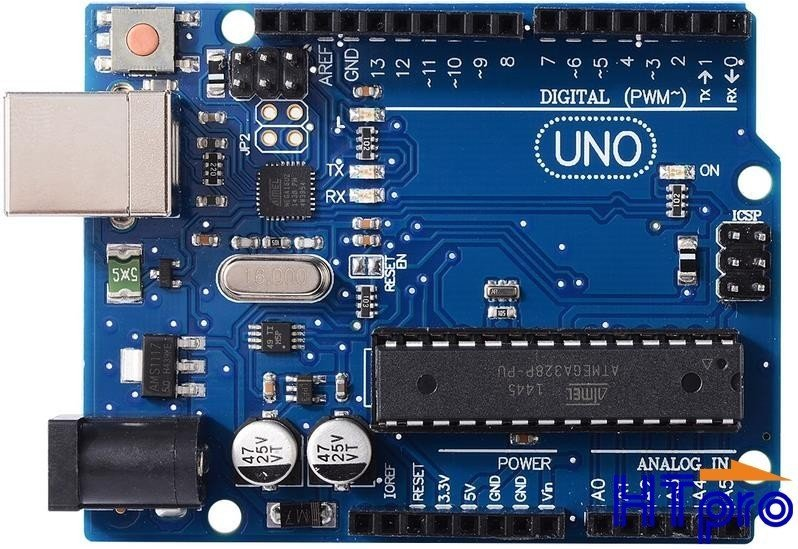
\includegraphics[width=0.5\linewidth]{image/adruino.jpg}
    \caption{Arduino Uno N3}
    % \label{fig:example1}
\end{figure}

\section{Cảm biến màu sắc}
Module cảm biến màu sắc sử dụng chip TCS3200. Led trắng có thể điều khiển bât hoặc tắt. Module có thể phát hiện màu sắc đối với vật không phát sáng, áp dụng để Phân loại màu sắc, Cảm biến ánh sáng xung quanh và hiệu chỉnh, phối hợp màu sắc.


\begin{itemize}[itemsep=0pt, parsep=0pt]
    \item Phát hiện màu sắc tĩnh, đầu ra là xung vuông với tần số tỷ lệ thuận với cường độ ánh sáng tới.
    \item Hỗ trợ ánh sáng bằng các đèn LED trên board mạch.
    \item Chuyển đổi từ cường độ ánh sáng sang tần số với độ phân giải cao.
    \item Lập trình lựa chọn bộ lọc màu sắc khác nhau và dạng tần số xuất ra.
    \item Điện năng tiêu thụ thấp. Giao tiếp trực tiếp với vi điều khiển.
\end{itemize}


\begin{figure}[H]
    \centering
    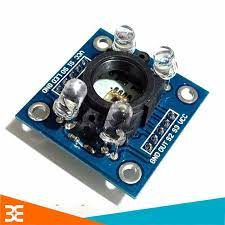
\includegraphics[width=0.4\linewidth]{image/sensor.jpg}
    \caption{Sensor TCS3200 V2}
    % \label{fig:example2}
\end{figure}

\section{Động cơ servo SG90}
Động cơ servo SG90 có kích thước nhỏ, là loại được sử dụng nhiều nhất để làm các mô hình nhỏ hoặc các cơ cấu kéo không cần đến lực nặng.
    \begin{figure}[H]
        \centering
        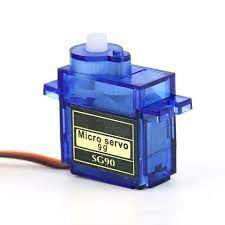
\includegraphics[width=0.5\linewidth]{image/servo.jpg}
        \caption{Động cơ servo SG90}
        % \label{fig:example3}
    \end{figure}
    
    \begin{table}[H] % Môi trường table để đánh số và đặt chú thích cho bảng
        \centering % Căn giữa bảng
        \begin{tabular}{ll} % Số "l" tương ứng với số cột trong bảng, có thể thay đổi thành "c" hoặc "r" để căn giữa hoặc căn phải
            \toprule % Đường kẻ đầu bảng
            Thông số & Giá trị \\
            \midrule % Đường kẻ giữa bảng
            Điện áp hoạt động & 4.8-5VDC \\
            Tốc độ & 0.12 sec/60 degrees (ở 4.8VDC) \\
            Lực kéo & 1.6KG.CM \\
            Kích thước & 21x12x22mm \\
            Trọng lượng & 9g \\
            \bottomrule % Đường kẻ cuối bảng
        \end{tabular}
        \caption{Bảng thông số kỹ thuật} % Chú thích cho bảng
        % \label{tab:thongso4} % Nhãn cho bảng để tham chiếu trong văn bản
    \end{table}


\section{Step motor NEMA 17}
Động cơ bước 17HS1538-1704A là loại động cơ bước hỗn hợp, có góc bước 1.8° và kích thước 40x42x42mm. Nó có 4 dây, mô-men xoắn giữ 0.45Nm, khả năng cung cấp moment xoắn cực lớn ở dải vận tốc thấp và trung bình.


\begin{center}
    \begin{minipage}{0.45\textwidth}
        \centering
        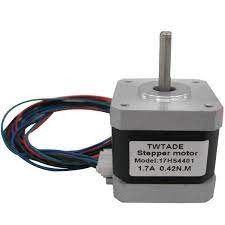
\includegraphics[width=\textwidth]{image/step_motor.jpg}
    \end{minipage}
    \hspace{0.05\textwidth}
    \begin{minipage}{0.45\textwidth}
        \centering
        \begin{tabular}{|c|c|}
            \hline
            Góc bước & 1.8° \\
            Mô-men xoắn & 0.45 Nm \\
            Số dây & 4 \\
            Điện áp & 12-24 V dc \\
            Kích thước & 40 x 42 x 42 mm \\
            Loại động cơ & Hỗn hợp \\
            Đường kính trục & 5 mm \\
            Dòng điện & 1.7 A \\
            Chiều dài trục & 23 mm \\
            Điện trở pha & 2.1 \\
            \hline
        \end{tabular}
    \end{minipage}
\end{center}

\section{Mạch Điều Khiển Động Cơ Bước A4988}
Mạch điều khiển động cơ bước A4988 là driver điều khiển động cơ bước cực kỳ nhỏ gọn, hỗ trợ nhiều chế độ làm việc, điều chỉnh được dòng ra cho động cơ, tự động ngắt điện khi quá nóng. Mạch điều khiển A4988 hỗ trợ nhiều chế độ hoạt động của động cơ bước lưỡng cực như: Full, 1/2, 1/4, 1/8 và 1/16.

    
    \begin{figure}[H]
        \centering
        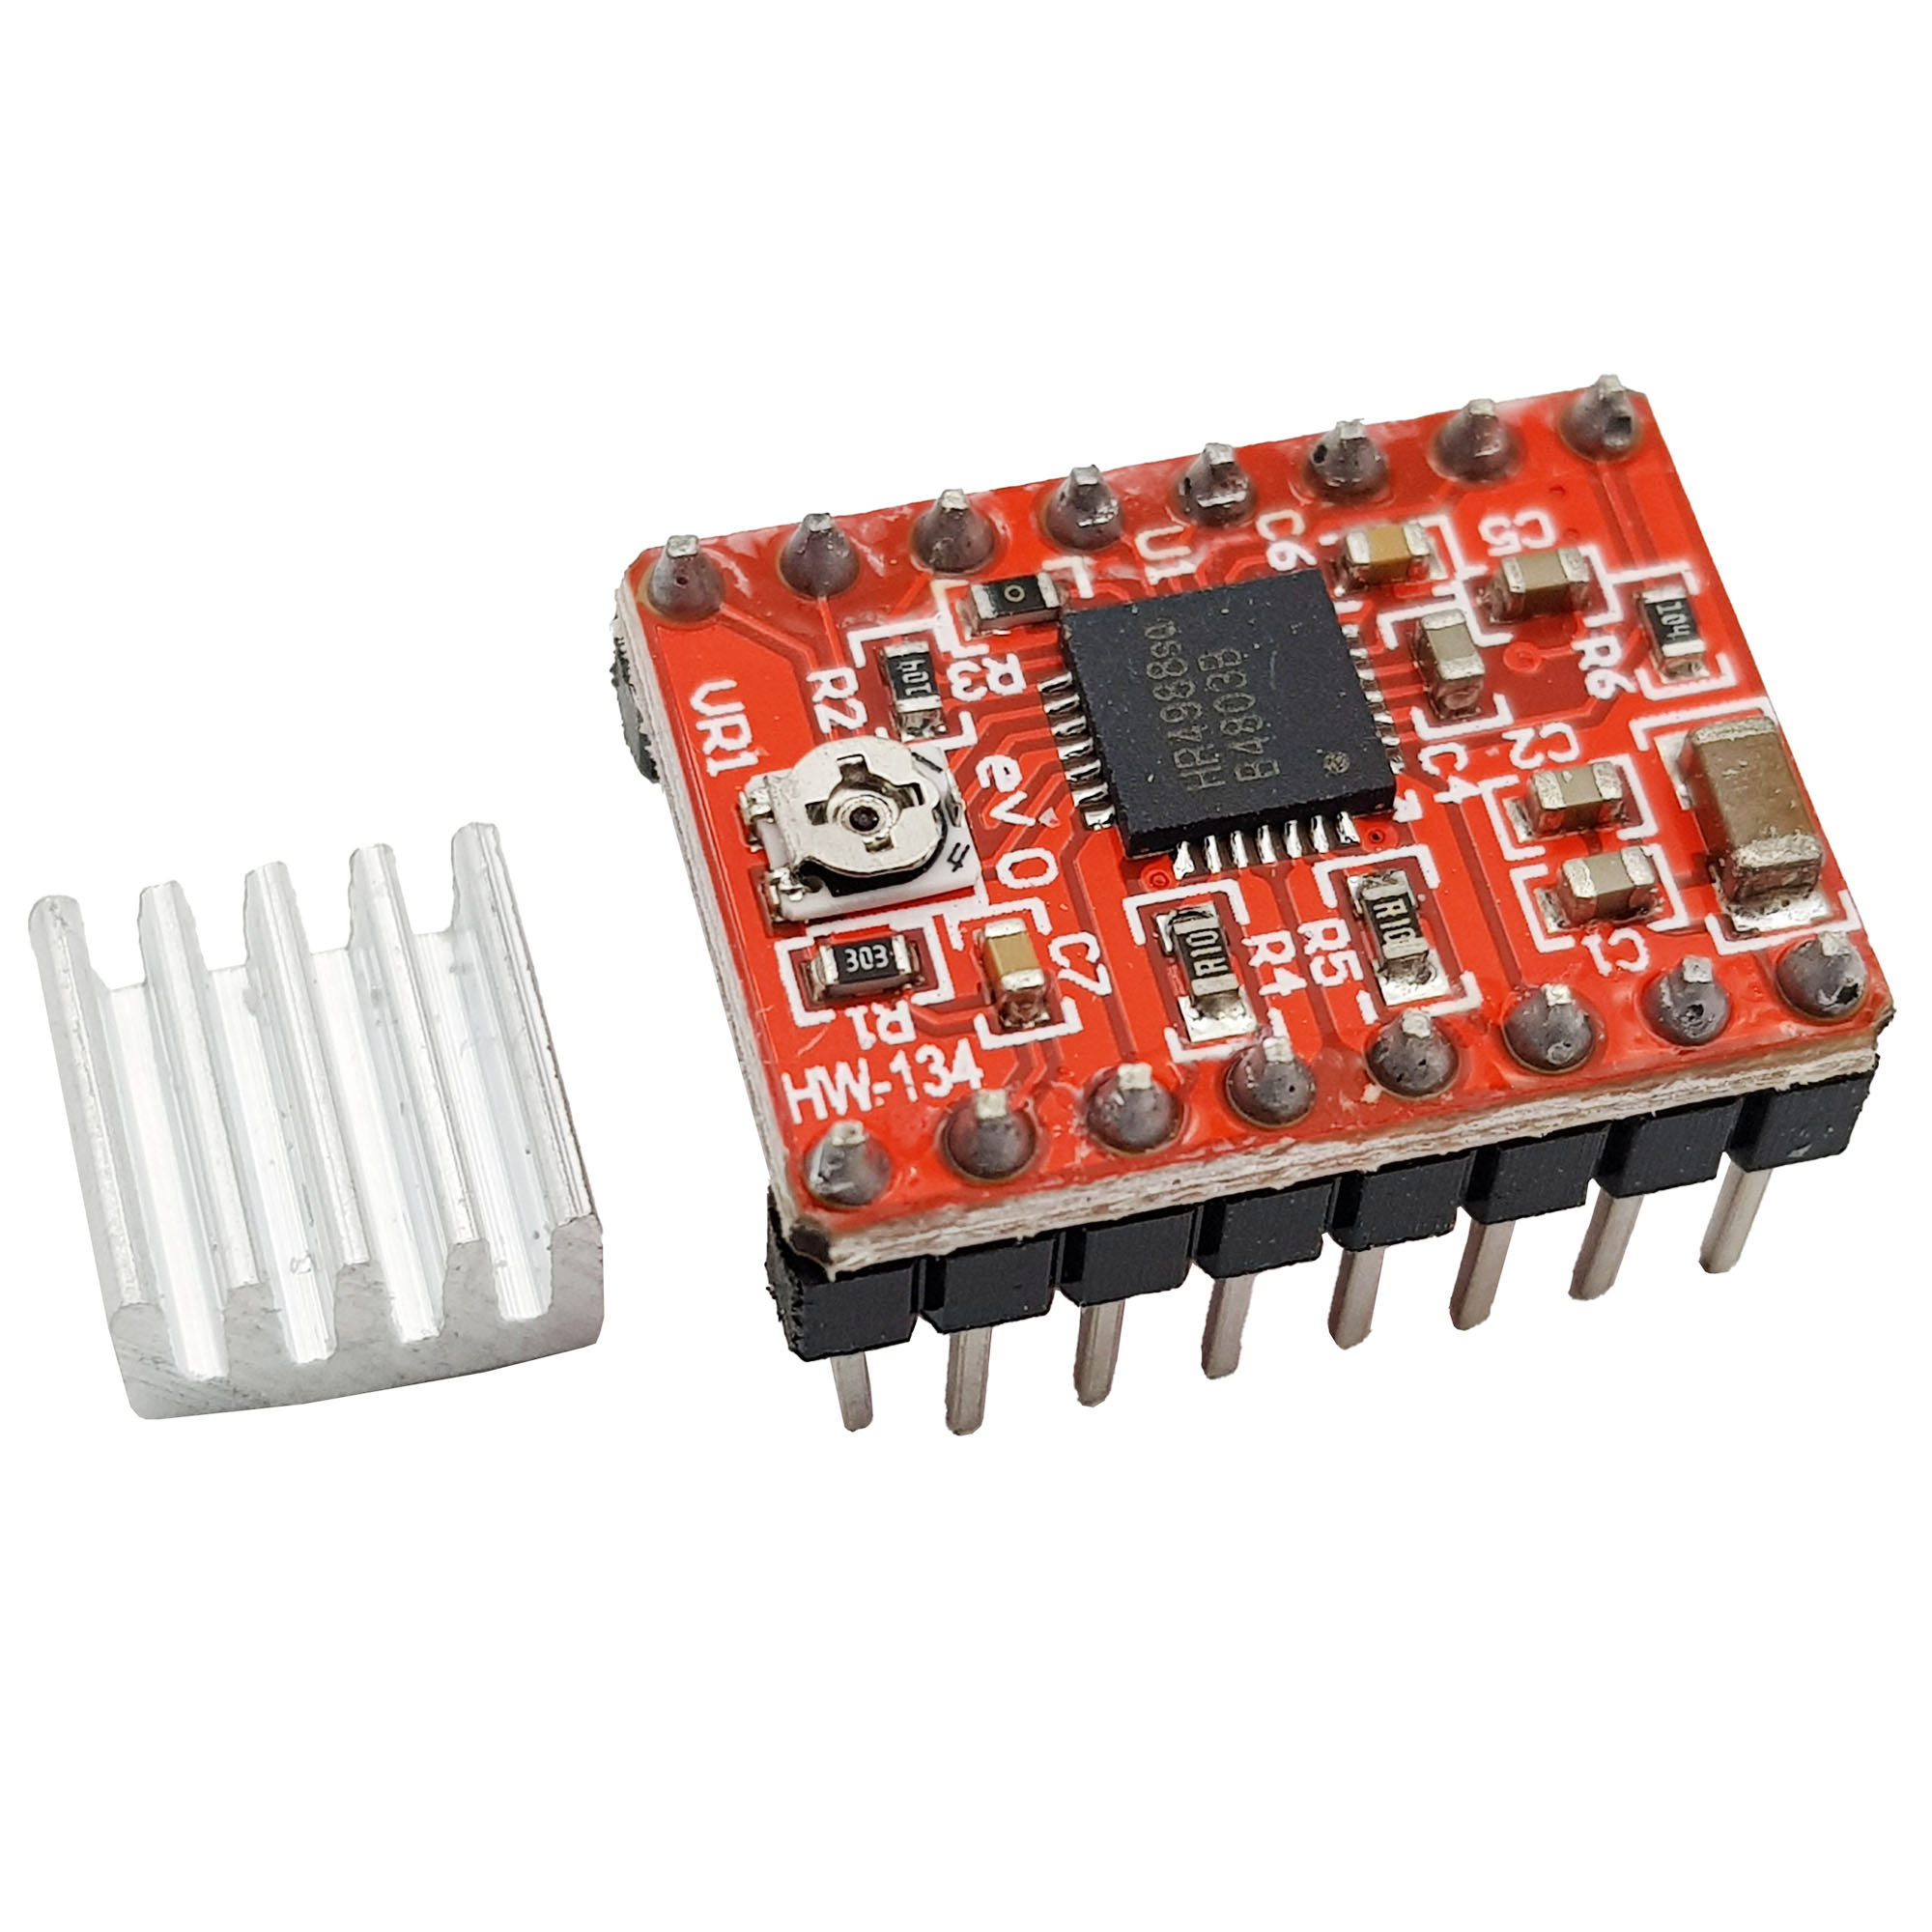
\includegraphics[width=0.5\linewidth]{image/driver.jpg}
        \caption{Mạch Điều Khiển Động Cơ Bước A4988}
        % \label{fig:example5}
    \end{figure}

\begin{table}[H]
    \centering
    \begin{tabular}{ll}
        \toprule % Đường kẻ đầu bảng
        Thông số & Giá trị \\
        \midrule % Đường kẻ giữa bảng
        Điện áp cấp tối thiểu & 8 V \\
        Điện áp cấp cực đại & 35 V \\
        Dòng cấp liên tục (không làm mát) & 1 A \\
        Dòng cấp liên tục (có làm mát, tản nhiệt) & 2 A \\
        Điện áp logic 1 tối thiểu & 3 V \\
        Điện áp logic 1 tối đa & 5.5 V \\
        Độ phân giải & full, 1/2, 1/4, 1/8, và 1/16 \\
        \bottomrule % Đường kẻ cuối bảng
    \end{tabular}
    \caption{Bảng thông số kỹ thuật} % Chú thích cho bảng
    % \label{tab:thongso2} % Nhãn cho bảng để tham chiếu trong văn bản
\end{table}

\chapter{MÔ HÌNH ĐẾM VÀ PHÂN LOẠI SẢN PHẨM}
\section{Các phân mềm thiết kế}

\subsection{Arduino IDE}
Arduino là môi trường phát triển tích hợp mã nguồn mở, cho phép người dùng dễ dàng viết code và tải nó lên board mạch, được viết bằng Java dựa trên ngôn ngữ lập trình và phần mềm mã nguồn mở khác.

    \begin{figure}[H]
        \centering
        
\includegraphics[width=0.5\linewidth]{image/arduino_ide.png}
        \caption{Phần mềm điều khiển Arduino}
        % \label{fig:example5}
    \end{figure}
    
Kể từ tháng 3 năm 2015, Arduino IDE (Intergrated Devalopment Editor – môi
trường phát triển thích hợp) đã được phổ biến tại rất nhiều nơi với giao diện trực quan.
Ngôn ngữ phổ quát cho Arduino là C và C++. Do đó phần mềm phù hợp với những người dùng quen thuộc các ngôn ngữ này.
Phần mềm gồm những mảng thư viện phong phú như: EEPROM, Firmata, GSM, Servo, TFT, Wifi,... Và các mảng thư viện ngày càng đa dạng nhờ sự đóng góp của cộng đồng Arduino trên toàn thế giới

\subsection{WinForms - Visual Studio}
Trong Visual Studio, bạn có thể tạo các dự án WinForms mới và thiết kế giao diện người dùng bằng giao diện kéo và thả. Bạn cũng có thể viết mã Logic để xử lý các sự kiện và tương tác với các thành phần giao diện của ứng dụng.

Visual Studio hỗ trợ nhiều ngôn ngữ lập trình như C, VB.NET, C++, và nhiều ngôn ngữ khác. Nó cũng hỗ trợ nhiều tích hợp và mở rộng bổ sung, giúp các nhà phát triển tăng cường hiệu suất và tối ưu hóa quá trình phát triển ứng dụng.

WinForms là một phần trong Microsoft .NET Framework, dùng để xây dựng ứng dụng desktop trên hệ điều hành Windows. WinForms cung cấp một bộ công cụ GUI (Giao diện người dùng đồ họa) cho các nhà phát triển, giúp họ thiết kế và xây dựng các giao diện ứng dụng Windows một cách dễ dàng.

WinForms hỗ trợ nhiều thành phần giao diện như các nút, ô văn bản, danh sách, menu, hộp thoại, và nhiều hơn nữa. Nhà phát triển có thể kéo và thả các thành phần này vào giao diện và sử dụng ngôn ngữ lập trình VB.NET để lập trình logic điều khiển các sự kiện và xử lý dữ liệu.


    \begin{figure}[H]
        \centering
        
\includegraphics[width=0.8\linewidth]{image/visual_studio.png}
        \caption{Visual Studio}
        % \label{fig:example6}
    \end{figure}

\subsection{Proteus 8 Professional}
Proteus là phần mềm mô phỏng mạch điện tử của Labcenter Electronics, mô phỏng cho hầu hết các linh kiện điện tử thông dụng, đặc biệt hỗ trợ cho cả các  PIC, 8051, AVR, ...
    \begin{figure}[H]
        \centering
        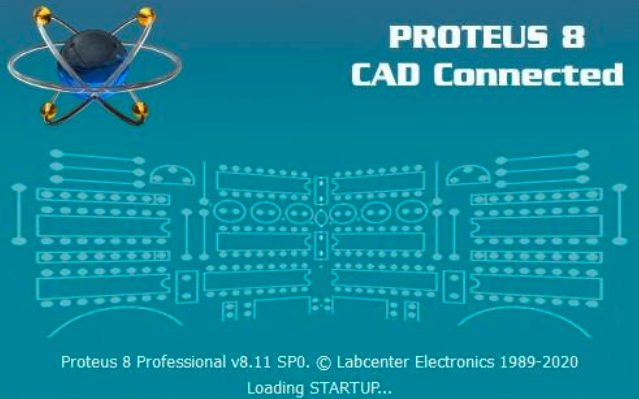
\includegraphics[width=0.5\linewidth]{image/proteus.png}
        \caption{Phần mềm proteus}
        % \label{fig:example0}
    \end{figure}

    
\section{Sơ đồ khối}
\begin{center}
    \begin{tikzpicture}[node distance=2cm, auto]
        % Define block styles
        \tikzstyle{block} = [rectangle, draw, text width=5em, text centered, minimum height=3em]
        \tikzstyle{line} = [draw, -latex]
        
        % Nodes
        \node [block] (source) {Khối nguồn};
        \node [block, below of=source] (display) {Khối tín hiệu};
        \node [block, below of=display] (classification) {Khối xử lý};
        \node [block, below of=classification] (sensors) {Khối phân loại};
        \node [block, below of=sensors] (processing) {Khối hiển thị};
        
        % Arrows
        \path [line] (source) -- (display);
        \path [line] (display) -- (classification);
        \path [line] (classification) -- (sensors);
        \path [line] (sensors) -- (processing);
        
        % Text labels
        \node [left of=source, xshift=-1.5cm] (input) {Đầu vào};
        \node [right of=processing, xshift=1.5cm] (output) {Đầu ra};
        \path [line] (input) -- (source);
        \path [line] (processing) -- (output);
        
    \end{tikzpicture}
\end{center}

\begin{itemize}[itemsep=0pt, parsep=0pt]
    \item \textbf{Khối nguồn gồm các linh kiện tác động đến công suất, dòng điện. (adapter, module nguồn):} Cung cấp năng lượng thích hợp cho mô hình hệ thống

    \begin{figure}[H]
        \centering
        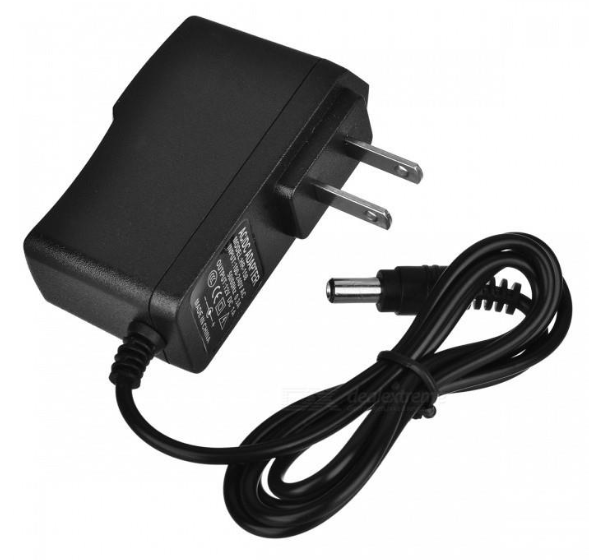
\includegraphics[width=0.5\linewidth]{image/KhoiNguon.png}
        \caption{Adapter 12V để cấp nguồn cho động cơ bước}
        % \label{fig:example9}
    \end{figure}
    
    \item \textbf{Khối hiển thị (Winform):} hiển thị số lượng đếm được từ cảm biến

    \begin{figure}[H]
        \centering
        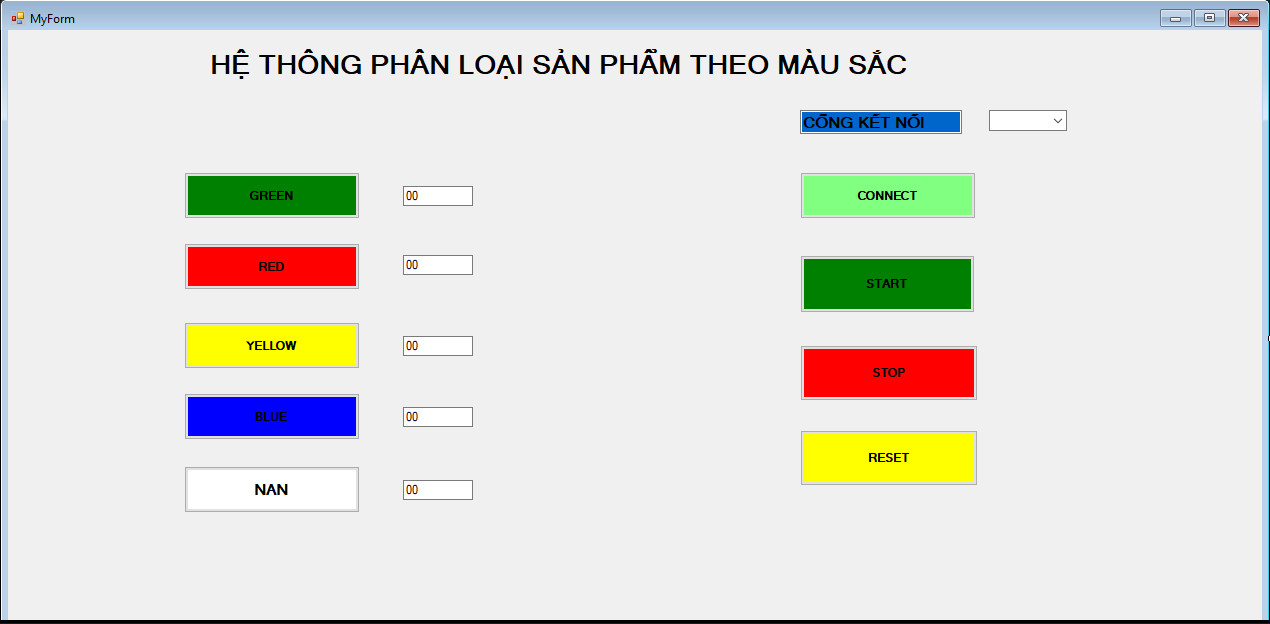
\includegraphics[width=1\linewidth]{image/KhoiGiaoDien.jpg}
        \caption{Giao diện điều khiển}
        % \label{fig:example10}
    \end{figure}
    
    \item \textbf{Khối phân loại (Động cơ bước, Servo):} phân các sản phẩm thành nhiều loại theo yêu cầu của mô hình đề tài.
    
    \item \textbf{Khối tín hiệu là các cảm biến màu sắc:} phát hiện màu sắc của vật thể và truyền tín hiệu về khối xử lý để mã hóa dữ liệu.
    
    \item \textbf{Khối xử lý (Arduino Uno R3, ...):} xử lý tín hiệu từ cảm biến và xuất dữ liệu được mã hóa đến các khối hiển thị, khối phân loại.
    
\end{itemize}

\section{Nguyên lý hoạt động}
    \begin{figure}[H]
        \centering
        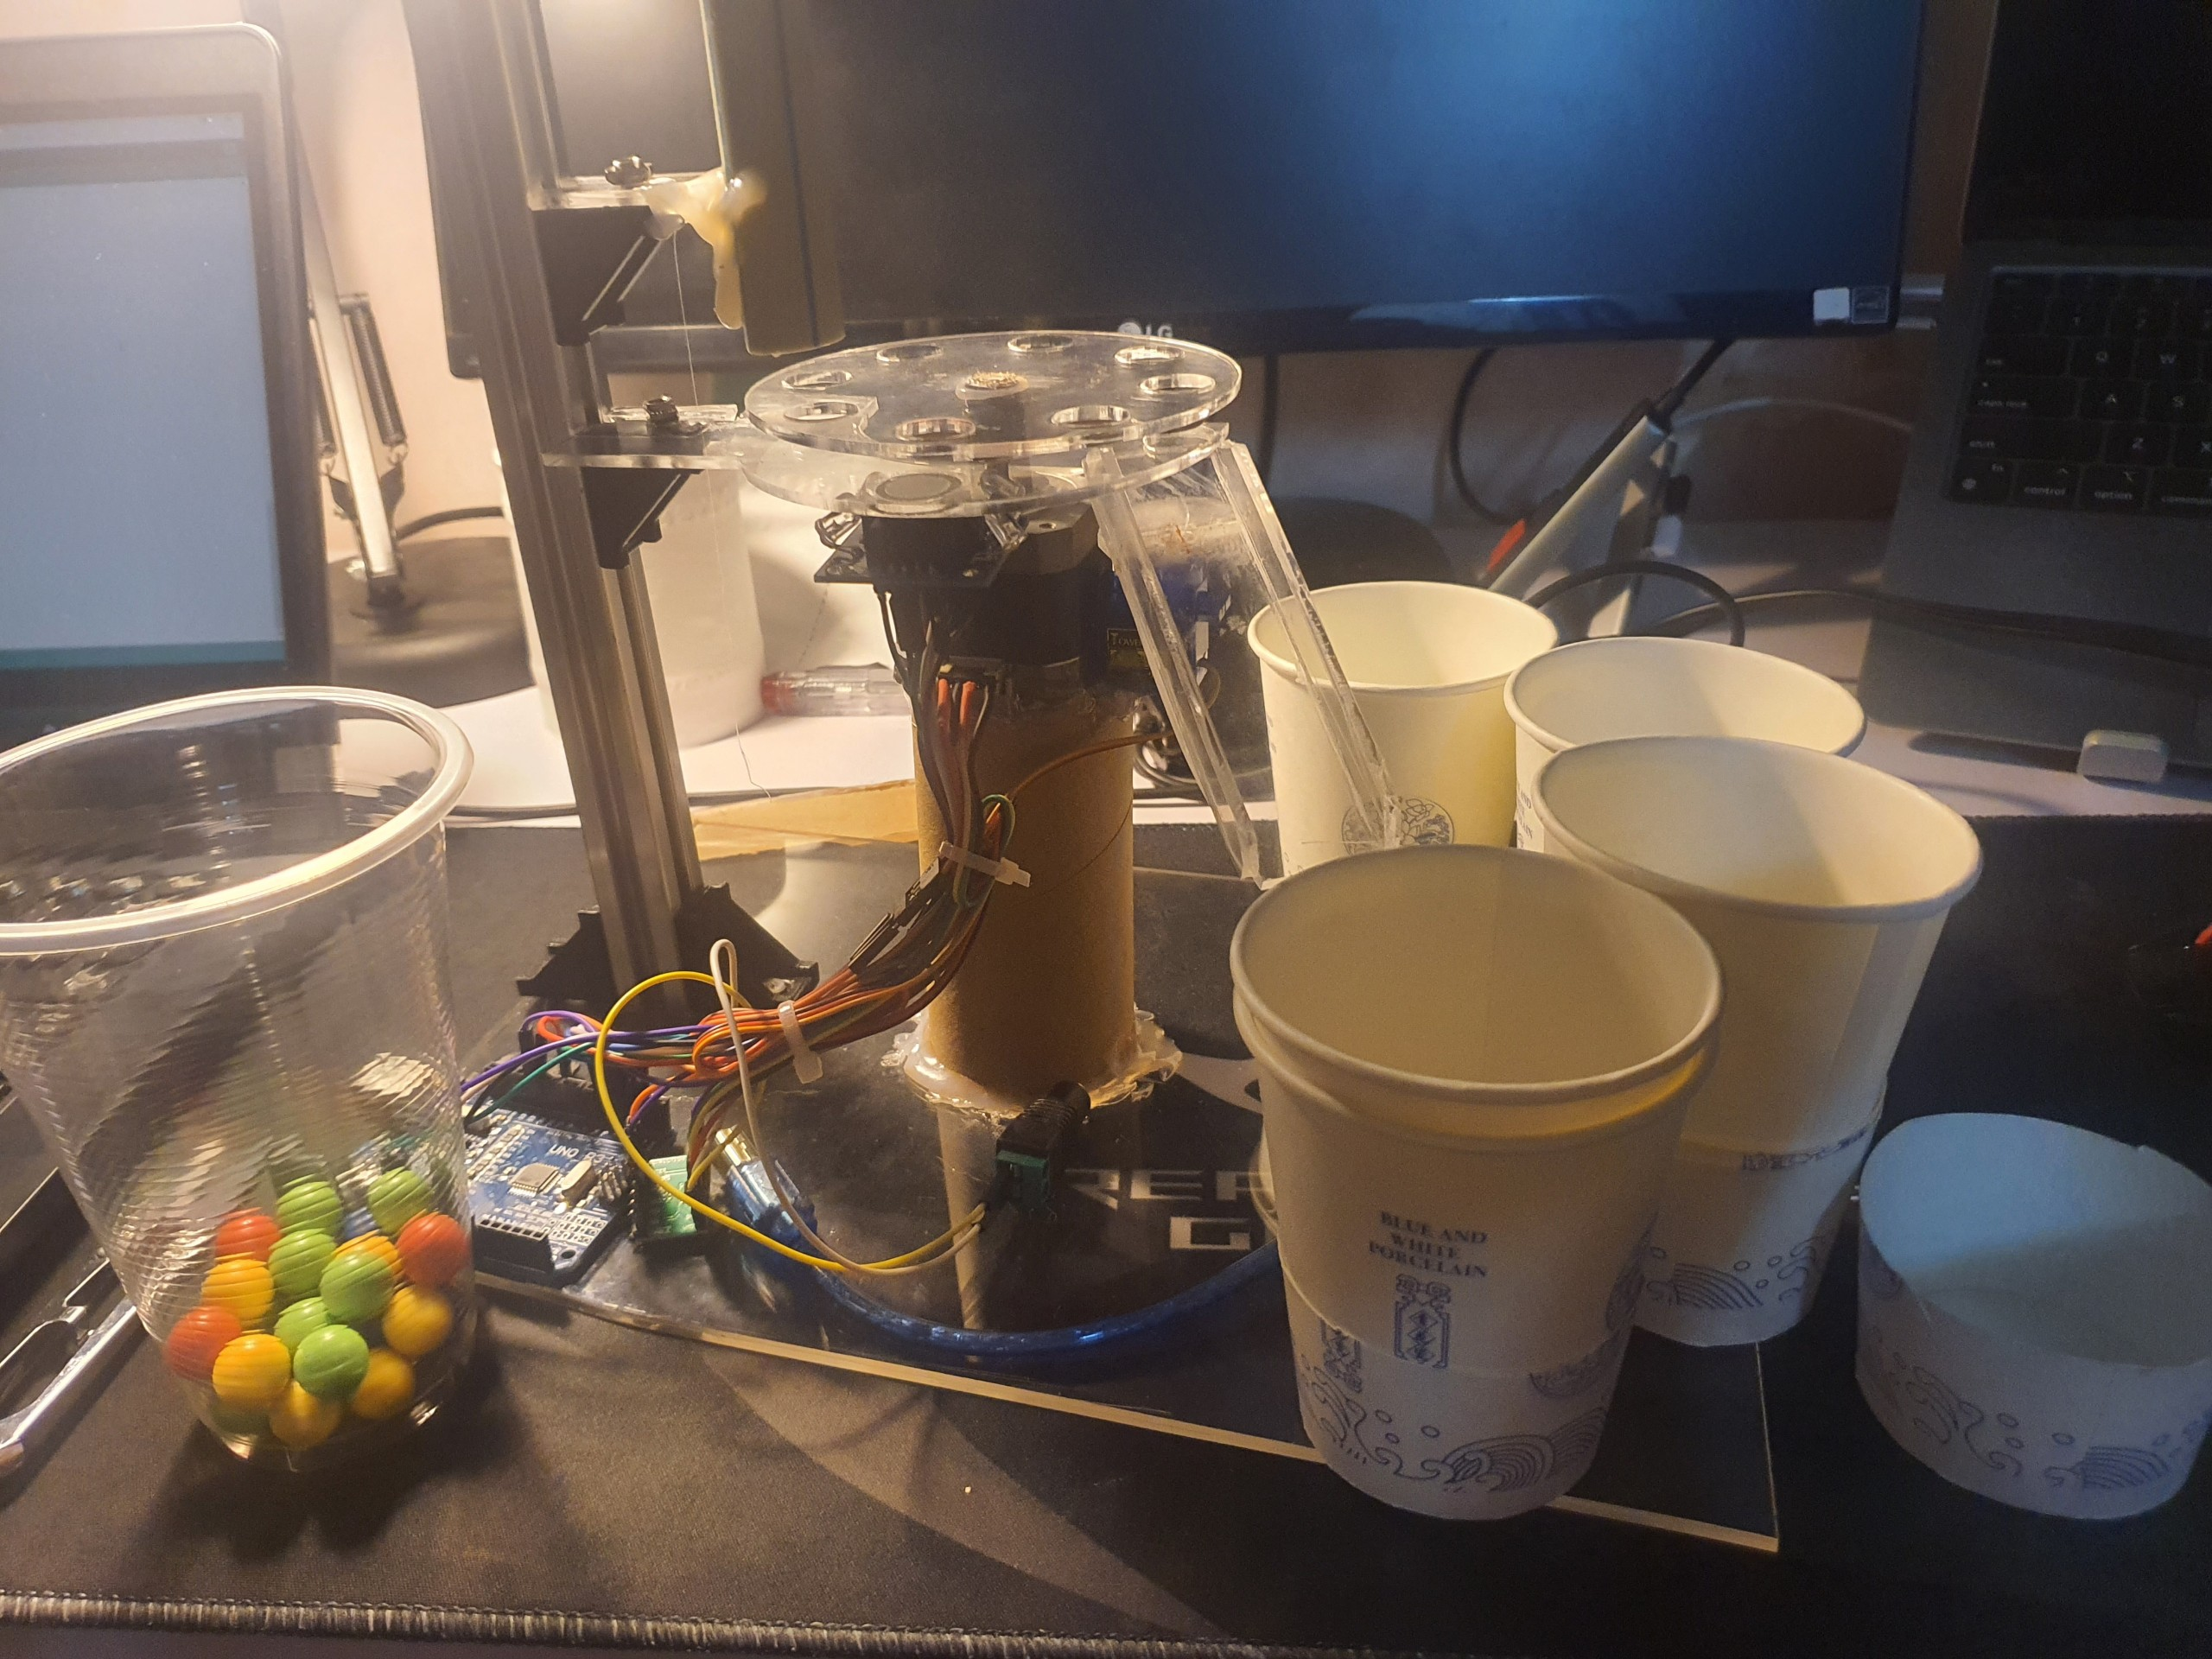
\includegraphics[width=1\linewidth]{image/mohinh.jpg}
        \caption{Mô hình thiết bị}
        % \label{fig:example}
    \end{figure}
    
    \begin{enumerate}[label=\arabic*., itemsep=0pt, parsep=0pt]
        \item \textbf{Sử dụng giao diện đồ hoạ để điều khiển:} Điều khiển kết nối với arduino và hệ thống bằng giao diện điều hoạ, ấn bắt đầu bằng bắt đầu 
        \item \textbf{Thu thập dữ liệu màu sắc:} Hệ thống sử dụng các cảm biến màu sắc để thu thập dữ liệu về màu sắc của các sản phẩm. Cảm biến này có thể sử dụng cảm biến RGB (Red-Green-Blue) để đo lường các giá trị màu cơ bản của vật thể.
        
        
        \item \textbf{Xử lý tín hiệu:} Dữ liệu điện thu được từ cảm biến màu sắc sẽ được xử lý bởi hệ thống xử lý (thường là vi điều khiển như Arduino). Hệ thống sẽ thực hiện việc xử lý tín hiệu và phân tích dữ liệu màu sắc để xác định màu của vật thể.
        
        \item \textbf{Phân loại sản phẩm:} Dựa vào kết quả đầu ra, hệ thống sẽ xác định xem sản phẩm thuộc màu sắc nào. Sau đó, hệ thống sẽ thực hiện các hành động tương ứng như điều khiển động cơ bước và quay servo các góc ứng với các màu để phân loại sản phẩm vào vị trí hoặc hộp tương ứng.
        
        \item \textbf{Hiển thị kết quả:} Cuối cùng, kết quả phân loại sản phẩm sẽ được hiển thị trên giao diện người dùng, thông qua màn hình hiển thị (WinForm).
    
    \end{enumerate}


\section{Lưu đồ thuật toán}
    \begin{figure}[H]
        \centering
        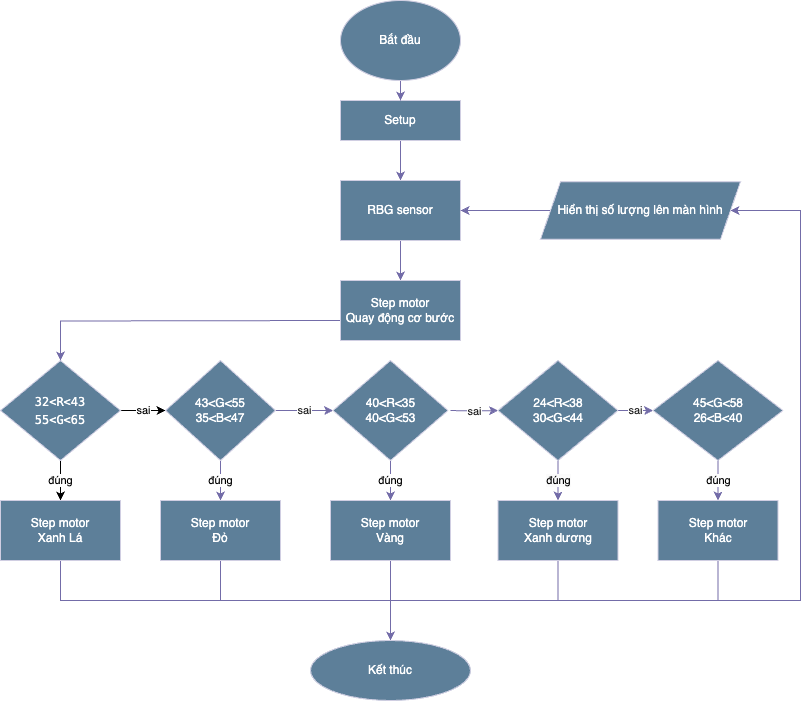
\includegraphics[width=1\linewidth]{image/Luudothuattoan.png}
        \caption{Lưu đồ thuật toán của hệ thống}
        % \label{fig:example}
    \end{figure}
\section{Code – chương trình}
\subsection*{Code aduino uno R3}
    \href{https://github.com/ngoxuanphong/arduino_color_sorting/blob/main/src/Color_Sorting_Arduino.ino}[Code aduino uno R3]
\subsection*{Code visual studio}
    \href{https://github.com/ngoxuanphong/arduino_color_sorting/blob/main/src/MyForm.h}[Code visual studio]

\chapter{Tổng kết}
\section{Ưu/ Nhược điểm}
\subsection*{Ưu điểm}

\begin{itemize}[itemsep=0pt, parsep=0pt]
    \item \textbf{Tự động hóa quy trình:} Hệ thống phân loại sản phẩm tự động hóa quy trình, giảm thiểu sự can thiệp của con người và tăng cường hiệu suất sản xuất.
    \item \textbf{Nhanh chóng và chính xác:} Hệ thống có thể phân loại sản phẩm nhanh chóng và chính xác dựa trên thông tin màu sắc, giảm thiểu sai sót và đảm bảo chất lượng sản phẩm.
    \item \textbf{Đa năng và linh hoạt:} Hệ thống có thể áp dụng trong nhiều lĩnh vực công nghiệp khác nhau và phân loại nhiều loại sản phẩm với độ phân giải khác nhau.
    \item \textbf{Tiết kiệm thời gian và chi phí:} Việc tự động hóa quy trình phân loại giúp tiết kiệm thời gian và giảm thiểu chi phí lao động.
    \item \textbf{Tích hợp dễ dàng vào hệ thống hiện có:} Hệ thống có kích thước nhỏ gọn và tích hợp dễ dàng vào các dây chuyền sản xuất hiện có.
\end{itemize}

\subsection*{Nhược điểm}

\begin{itemize}[itemsep=0pt, parsep=0pt]

    \item \textbf{Phụ thuộc vào môi trường:} Hiệu suất của hệ thống có thể bị ảnh hưởng bởi các yếu tố môi trường như ánh sáng, nhiệt độ và độ ẩm.
    \item \textbf{Khả năng phân loại hạn chế:} Hệ thống phân loại dựa trên thông tin màu sắc có thể gặp khó khăn khi phân loại các sản phẩm có sự tương đồng về màu sắc hoặc sự biến đổi về ánh sáng.

    \item \textbf{Hạn chế về độ chính xác:} Mặc dù hệ thống có thể đạt được độ chính xác cao, nhưng nó vẫn không thể thay thế hoàn toàn sự can thiệp và kiểm tra của con người trong một số trường hợp đặc biệt.
\end{itemize}
\section{Hướng phát triển} 
Hệ thống phân loại sản phẩm bằng màu sắc sử dụng cảm biến màu sắc và Arduino có thể phát triển và cải tiến theo các hướng sau:


\begin{itemize}[itemsep=0pt, parsep=0pt]
    \item \textbf{Nâng cao độ chính xác:} Tăng cường việc nghiên cứu và triển khai các thuật toán xử lý tín hiệu màu sắc để nâng cao độ chính xác trong quá trình phân loại sản phẩm. Có thể sử dụng các phương pháp học máy và trí tuệ nhân tạo để cải thiện khả năng phân loại.
    
    \item \textbf{Mở rộng ứng dụng:} Nghiên cứu và phát triển các ứng dụng mới cho hệ thống phân loại, bao gồm phân loại sản phẩm có kích thước và hình dạng đa dạng, từ đó mở rộng sự ứng dụng của hệ thống trong các lĩnh vực công nghiệp khác nhau.
    
    \item \textbf{Tối ưu hóa hiệu suất:} Nghiên cứu và tối ưu hóa quy trình phân loại sản phẩm, từ việc tăng tốc độ phân loại đến giảm thiểu thời gian phản hồi của hệ thống. Cải thiện hiệu suất giúp tăng năng suất sản xuất và giảm chi phí.
    
    \item \textbf{Mở rộng khả năng kết nối:} Nghiên cứu và phát triển khả năng kết nối hệ thống phân loại với các hệ thống quản lý và kiểm soát tự động khác, để tối ưu hóa quy trình sản xuất và tăng tính tự động hóa trong nhà máy.
    
    \item \textbf{Nâng cao tính ổn định và độ tin cậy:} Tối ưu hóa cấu trúc và các bộ phận của hệ thống để đảm bảo tính ổn định và độ tin cậy trong quá trình hoạt động. Điều này giúp tránh các sự cố và hỏng hóc trong quá trình sản xuất.
    
    \item \textbf{Phát triển giao diện người dùng:} Xây dựng một giao diện người dùng thân thiện và dễ sử dụng để tương tác với hệ thống phân loại. Giao diện này có thể hiển thị kết quả phân loại và các thông tin liên quan khác để người dùng có thể kiểm soát và giám sát hoạt động của hệ thống.
\end{itemize}

% \newpage
% \begin{thebibliography}{12}
%     \addcontentsline{toc}{chapter}{\quad\  \bf Tài liệu tham khảo}
%    \bibitem{1}Giáo trình kỹ thuật lập trình hệ cơ điện tử\\\textit{Trương Công Tuấn}
%    \bibitem{2}Module cảm biến màu sắc TCS3200\\ \href{https://github.com/Panjkrc/TCS3200_library}[Module cảm biến màu sắc]
%    \bibitem{3}Mạch điều khiển động cơ bước\\ \href{https://istem.com.vn/blog/dieu-khien-dong-co-buoc-voi-arduino-va-driver-a4988}[Mạch điều khiển động cơ bước]
%    \bibitem{4}Động cơ bước\\ \href{https://chuongmotor.com/dong-co-buoc-khai-niem-phan-loai-nguyen-ly-hoat-dong.html}[Động cơ bước]
%    \bibitem{5}Động cơ servo\\ \href{https://www.hwlibre.com/vi/servo-sg90/}[skittle color sorter]
%    \bibitem{6}Arduino UNO R3\\ \href{http://arduino.vn/bai-viet/42-arduino-uno-r3-la-gi}[Arduino UNO R3]
%    \bibitem{6}skittle color sorter yumin-chebn\\ \href{https://github.com/yumin-chen/skittle-color-sorter}[skittle color sorter]
% \end{thebibliography}

\end{document}
